\documentclass{standalone}
\usepackage{tikz}
\usepackage{ctex,siunitx}
\usepackage{tkz-euclide}
\usepackage{amsmath}
\usetikzlibrary{patterns, calc}
\usetikzlibrary {decorations.pathmorphing, decorations.pathreplacing, decorations.shapes,}
\begin{document}
\small
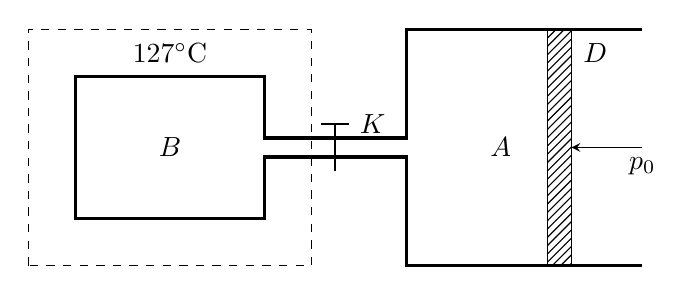
\begin{tikzpicture}[>=stealth,scale=0.6]
  \draw[very thick] (10, -2.5)--(5, -2.5)--(5,-.2)--(2, -.2)--(2, -1.5)--(-2, -1.5)--(-2, 1.5)--(2, 1.5)--(2, .2)--(5,.2)--(5, 2.5)--(10, 2.5);
  \draw[dashed](-3,-2.5) rectangle (3,2.5);
  \fill [pattern=north east lines, draw](8,-2.5) rectangle(8.5,2.5);
  \node at (0,2){127$^\circ$C}; \node at (9,2){$D$}; 
  \node at (0,0){$B$};  \node at (7,0){$A$};
  \draw [->](10,0)node [below]{$p_0$}--(8.5,0);
  \draw[thick](3.5,-.5)--(3.5,.5);
  \draw[thick](3.2,.5)--(3.8,.5)node[right]{$K$};
\end{tikzpicture}
\end{document}